\documentclass{standalone}
\usepackage{tikz}
\usetikzlibrary{3d,arrows, calc, backgrounds, petri, positioning, shapes.geometric}

\tikzset{
	persp/.style={scale=3.0,x={(-0.8cm,-0.4cm)},y={(0.8cm,-0.4cm)}, z={(0cm,1cm)}},
	points/.style={fill=white,draw=black,thick}
	grid/.style={very thin,gray},
	axis/.style={->,blue,ultra thick},
	cube/.style={thick, fill=black!15,opacity=0.5},
	cube hidden/.style={dashed},
	block/.style={
		rectangle, rounded corners,
		draw=black!80,
		fill=black!10, fill opacity=0.5,
		text=black!90, text opacity=1.0,
    text height=1.5ex,
    text depth=.25ex,
    text width=6em,
    text centered
	}
}

\newcommand*{\rootPath}{../}

\begin{document}
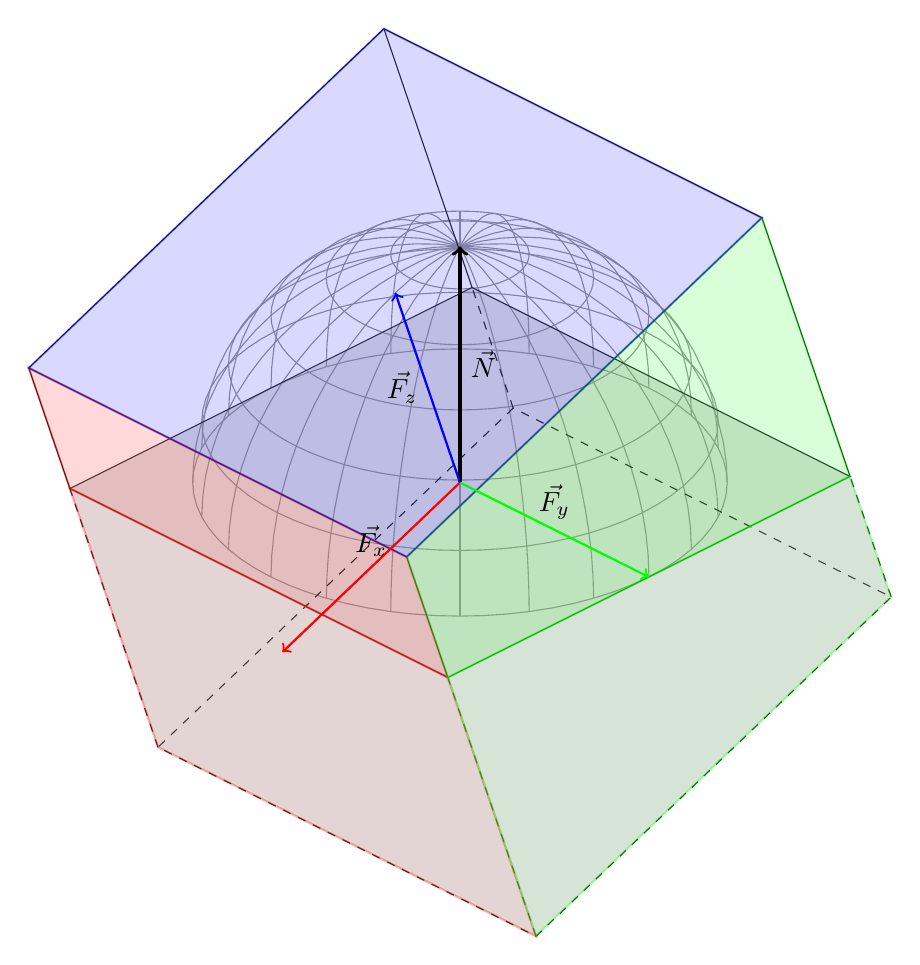
\begin{tikzpicture}[persp]
	\def\i{-20}
	\pgfmathparse{cos(\i)}\let\ci\pgfmathresult
	\pgfmathparse{sin(\i)}\let\si\pgfmathresult
	\coordinate	(Ocube)	at (0,0,0);
	\coordinate	(Xcube)	at (\ci,0,\si);
	\coordinate	(Ycube)	at (0,1,0);
	\coordinate	(Zcube)	at (-\si,0,\ci);
	\coordinate (A) at ($(Ocube)-(Xcube)-(Ycube)-(Zcube)$);
	\coordinate (B) at ($(Ocube)+(Xcube)-(Ycube)-(Zcube)$);
	\coordinate (C) at ($(Ocube)-(Xcube)+(Ycube)-(Zcube)$);
	\coordinate (D) at ($(Ocube)+(Xcube)+(Ycube)-(Zcube)$);
	\coordinate (E) at ($(Ocube)-(Xcube)-(Ycube)+(Zcube)$);
	\coordinate (F) at ($(Ocube)+(Xcube)-(Ycube)+(Zcube)$);
	\coordinate (G) at ($(Ocube)-(Xcube)+(Ycube)+(Zcube)$);
	\coordinate (H) at ($(Ocube)+(Xcube)+(Ycube)+(Zcube)$);
	\coordinate (OA) at (-1.0/\ci,-1.0,+0.0);
	\coordinate (OB) at (+1.0/\ci,-1.0,+0.0);
	\coordinate (OC) at (-1.0/\ci,+1.0,+0.0);
	\coordinate (OD) at (+1.0/\ci,+1.0,+0.0);
	\fill[black!15] (OA)--(OB)--(B)--(D)--(C)--(OC)--cycle;
	\foreach \t in {0,15,...,165}
	{
		\draw[gray] ({cos(\t)},{sin(\t)},0)
		\foreach \rho in {5,10,...,180}
			{--({cos(\t)*cos(\rho)},{sin(\t)*cos(\rho)},{sin(\rho)})};
	}
	\foreach \t in {0,15,...,75}
	{
		\draw[gray] ({cos(\t)},0,{sin(\t)})
		\foreach \rho in {5,10,...,355}
			{--({cos(\t)*cos(\rho)},{cos(\t)*sin(\rho)},{sin(\t)})}--cycle;
	}
	\draw[dashed]	(A)--(B)--(D)--(C)--cycle;
	\draw			(OA)--(OB)--(OD)--(OC)--cycle;
	\draw			(E)--(F)--(H)--(G)--cycle;
	\draw[dashed]	(A)--(OA) (B)--(OB) (C)--(OC) (D)--(OD);
	\draw			(E)--(OA) (F)--(OB) (G)--(OC) (H)--(OD);
	\fill[red!50,	draw=red,	thick,opacity=0.3] (OB)--(OD)--(H)--(F)--cycle;
	\fill[red!20,	draw=red,	thick,opacity=0.3] (B)--(D)--(OD)--(OB)--cycle;
	\fill[green!50,	draw=green,	thick,opacity=0.3] (OC)--(OD)--(H)--(G)--cycle;
	\fill[green!20,	draw=green,	thick,opacity=0.3] (C)--(D)--(OD)--(OC)--cycle;
	\fill[blue!50,	draw=blue,	thick,opacity=0.3] (E)--(F)--(H)--(G)--cycle;
	\draw[->,very thick,black]	(Ocube)--(0,0,1)	node[black,midway,right]	{$\vec{N}$};
	\draw[->,thick,red]			(Ocube)--(Xcube)	node[black,midway,above]	{$\vec{F_x}$};
	\draw[->,thick,green]		(Ocube)--(Ycube)	node[black,midway,above]	{$\vec{F_y}$};
	\draw[->,thick,blue]		(Ocube)--(Zcube)	node[black,midway,left]		{$\vec{F_z}$};
\end{tikzpicture}
\end{document}
